\documentclass[12pt,class=article,crop=false,preview=false]{standalone}

\usepackage[utf8]{inputenc}

\usepackage{amsmath}
\usepackage{amssymb}
\usepackage{siunitx}
\sisetup{range-phrase=--}
\sisetup{range-units=single}
\sisetup{per-mode=symbol}

\usepackage{xcolor}
\usepackage[unicode]{hyperref}
\usepackage{minted}
\usepackage{fullpage}

\usepackage{tikz}
\usepackage[siunitx]{circuitikz}
\usepackage{tikz-3dplot}

\tdplotsetmaincoords{110}{-12}
\usetikzlibrary {arrows.meta}
\usepackage{stanli}

\usepackage{enumitem}

\newcommand{\mat}[1]{\left[\begin{matrix}#1\end{matrix}\right]}
\newcommand{\vectwo}[2]{\left[\begin{matrix}#1\\#2\end{matrix}\right]}
\newcommand{\mattwo}[4]{\left[\begin{matrix}#1 & #3\\#2 & #4\end{matrix}\right]}

\DeclareMathOperator{\dive}{div}
\DeclareMathOperator{\grad}{grad}
\DeclareMathOperator{\tr}{tr}

\newcommand{\rr}[2]{\frac{\partial #1}{\partial #2}}
\newcommand{\pr}[1]{\frac{\partial}{\partial #1}}
\newtheorem{exercise}{Exercise}[section]

\usepackage{comment}
\specialcomment{solution}{{\bf Solution}\quad}{}

\setcounter{section}{2}
%\excludecomment{solution}

\begin{document}
\subsection*{Exercises}

\begin{exercise}
For a element size $h$ and four points $p^0=\{0,0\}$, $p^1=\{h,0\}$, $p^2=\{0,h\}$, $p^3=\{h,h\}$ forming a square in 2D:
\begin{enumerate}[label=\alph*)]
\item check what is the minimal order of a polynomial, which could would evaluate to $1$ on one of the points and $0$ on remaining three.
\item propose four such functions $\phi_i$, each evaluating to $1$ on the corresponding point $p_i$.
\item Compute $\int_\square\phi_i\phi_j$ for every pair of $i$ and $j$. Are there any symmetries you can exploit?
\item Compute $\int_\square \left(\rr{\phi_i}{x}\rr{\phi_j}{x} + \rr{\phi_i}{y}\rr{\phi_j}{y}\right)$
\end{enumerate}
\end{exercise}

\begin{solution}
We need a polynomial of minimum 2nd order, otherwise we don't have enough coefficients. The 2nd order polynomial in 2d is:
\[g(x,y)=a+bx+cy+dx^2+ey^2+fxy\]
(option 1) We can directly say here that we have too many coefficients (we have 6 coefficients and only 4 equations) and remove some. If one tries to remove $f$ the equations won't work, so he will conclude that $d$ and $e$ are to be removed.

(option 2) We can go with all coefficients and get rid of them later. For a), the easiest case to do is having 1 in $p^3$ and 0 in other three (but it's not much harder for other cases):
\begin{align*}
    g(p^0)&=g(0,0)=&a &= 0\\
    g(p^1)&=g(h,0)=&a+bh+dh^2 &= 0\\
    g(p^2)&=g(0,h)=&a+ch+eh^2 &= 0\\
    g(p^2)&=g(h,h)=&a+bh+ch+dh^2+eh^2+fh^2 &= 1\\
\end{align*}
This gives us: $a=0$, $b = -dh$, $c = -eh$ and $f=\frac{1}{h^2}$. Here we see that we have a freedom of choice of $d$ and $e$, and we can just set them to $0$ to simplify our function.

Finally we get $g(x,y) = \frac{1}{h^2}xy$, and we can solve b) by simple flipping of this function (or solving an analogous problem like before):
\[\phi_0(x,y)=\frac{1}{h^2}(h-x)(h-y)\quad\phi_1(x,y)=\frac{1}{h^2}x(h-y)\quad\phi_2(x,y)=\frac{1}{h^2}(h-x)y\quad\phi_3(x,y)=\frac{1}{h^2}xy\]

For c), let us first consider the simplest case of $i=3$, $j=3$:
\[\int_\square\phi_3\phi_3 = \int_0^h\int_0^h\frac{1}{h^2}xy\frac{1}{h^2}xydydx = \frac{1}{h^4}\int_0^h\int_0^h x^2y^2dydx = \frac{1}{h^4}\int_0^h x^2dx\int_0^hy^2dy = \frac{1}{h^4}\frac{h^3}{3}\frac{h^3}{3} = \frac{1}{9}h^2\]
Students who didn't hone their integration skills can always use the power of the internet:
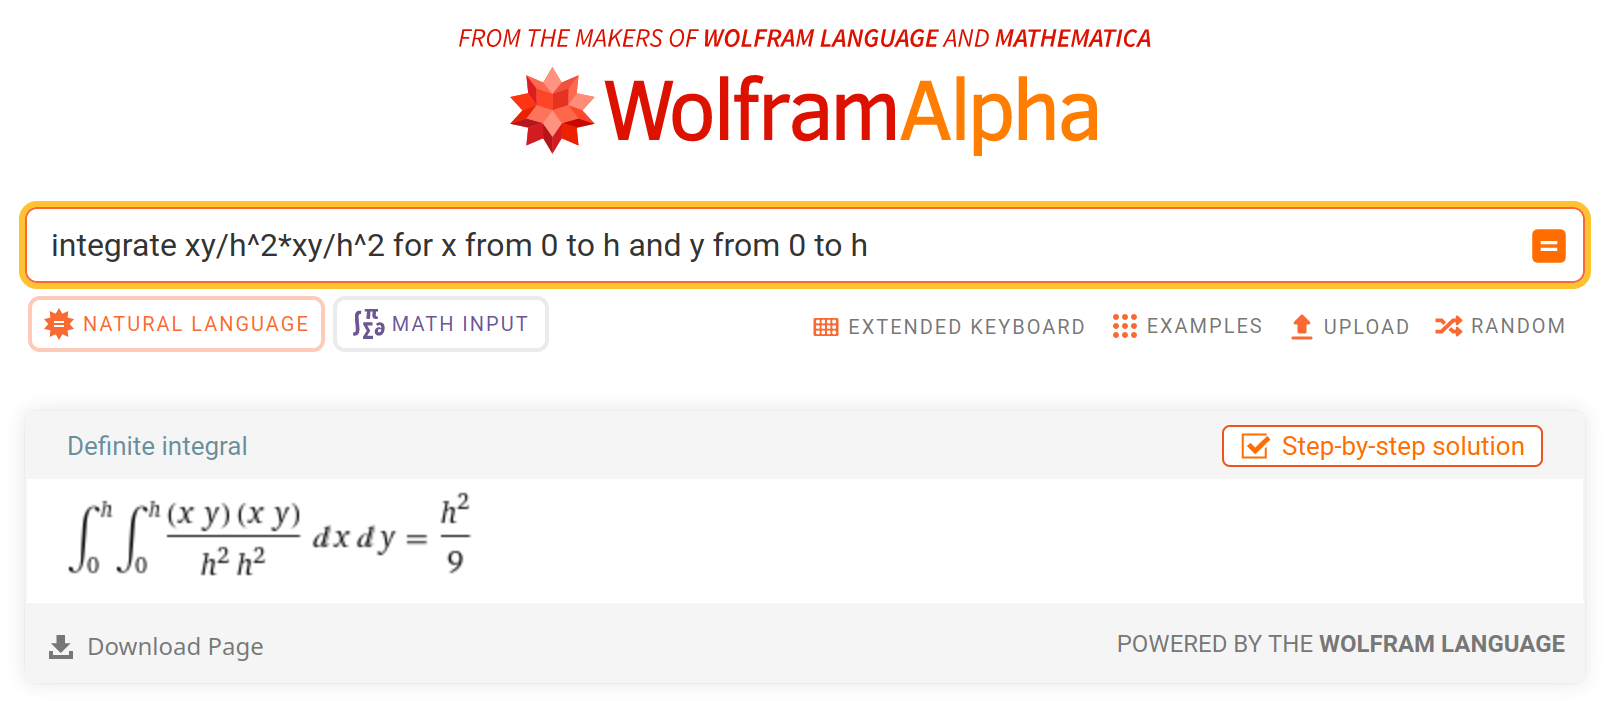
\includegraphics[width=\textwidth]{img/integral1.png}
Same way you can compute that: $\int_\square\phi_2\phi_3 = \frac{h^2}{18}$ and $\int_\square\phi_1\phi_3 = \frac{h^2}{36}$. Finally by symmetry we can write out all the integrals as a matrix:
\[\mat{\int_\square\phi_i\phi_j} = h^2\mat{
\frac{1}{9} & \frac{1}{18} & \frac{1}{18} & \frac{1}{36}\\
\frac{1}{18} & \frac{1}{9} & \frac{1}{36} & \frac{1}{18}\\
\frac{1}{18} & \frac{1}{36} & \frac{1}{9} & \frac{1}{18}\\
\frac{1}{36} & \frac{1}{18} & \frac{1}{18} & \frac{1}{9}} = \frac{h^2}{36}\mat{
4 & 2 & 2 & 1\\
2 & 4 & 1 & 2\\
2 & 1 & 4 & 2\\
1 & 2 & 2 & 4}\]

For d), one has to compute the derivatives of the $\phi$ functions:
\begin{align*}
    \grad\phi_0 &= \frac{1}{h^2}[-(h-y),-(h-x)] & \grad\phi_1 &= \frac{1}{h^2}[(h-y),-x]\\
    \grad\phi_2 &= \frac{1}{h^2}[-y,(h-x)] & \grad\phi_3 &= \frac{1}{h^2}[y,x]
\end{align*}
Again the simplest case is the one with $i=3$, $j=3$:
\[\int_\square \left(\rr{\phi_i}{x}\rr{\phi_j}{x} + \rr{\phi_i}{y}\rr{\phi_j}{y}\right) = \int_\square \frac{1}{h^4}\left(y^2+x^2\right)= \frac{1}{h^4}\int_0^h\int_0^h \left(y^2+x^2\right)dydx=\frac{1}{h^4}\frac{2h^4}{3} = \frac{2}{3}\]
Same way one can compute the integral for $i=2$, $j=3$ to be $-\frac{1}{6}$, and for $i=1$, $j=3$ to be $-\frac{1}{3}$. Finally the matrix of the integrals is:
\[\mat{\int_\square \left(\rr{\phi_i}{x}\rr{\phi_j}{x} + \rr{\phi_i}{y}\rr{\phi_j}{y}\right)} = \frac{1}{6}\mat{
4 & -1 & -1 & -2\\
-1 & 4 & -2 & -1\\
-1 & -2 & 4 & -1\\
-2 & -1 & -1 & 4}\]
\end{solution}

\begin{exercise}
For a function $A:\mathbb{R}^{n\times n}\rightarrow\mathbb{R}^{n\times n}$ which takes a matrix and returns a matrix:
\[A(B) = \alpha B + \beta I \tr{B},\quad\text{(reminder: $\tr{B}=\sum_iB_{ii}$)}\]
show that for any matrix $C$:
\[C^{-1}A(B)C = A\big(C^{-1}BC\big)\]
\end{exercise}

\begin{solution}
    If one remembers from linear algebra, or looks it up on wikipedia:
    \[\tr XY = \tr YX\]
    This is because: $\tr XY = \sum_i\sum_j X_ijY_ji = \sum_j\sum_i Y_jiX_ij = \tr YX$. This is useful because $\tr {C^{-1}BC} = \tr {BCC^-1} = \tr B$ (which is also on wikipedia).

    
    That was the only ``problem'' on the exercise:
    \begin{align*}
    \text{left-hand-side} &= C^{-1}A(B)C = C^{-1}\big(\alpha B + \beta I \tr{B}\big)C
     = \alpha C^{-1}BC + \beta C^{-1}IC \tr{B}=\\&= \alpha C^{-1}BC + \beta I \tr{B}\\
    \text{right-hand-side} &= A\big(C^{-1}BC\big) = \alpha \big(C^{-1}BC\big) + \beta I \tr\big(C^{-1}BC\big) = \alpha C^{-1} B C + \beta I \tr B
    \end{align*}
\end{solution}

\begin{exercise}
For a function $f(x) = e^{\mathrm{i}kx}$ calculate:
\begin{enumerate}[label=\alph*)]
\item $f''(x)$
\item $\frac{f(x+h) - 2f(x) + f(x-h)}{h^2}$
\end{enumerate}
And compare the results. What can you say about these results for $f(x) = e^{-\mathrm{i}kx}$ and $f(x) = \cos{kx}$?
\end{exercise}
\newcommand{\im}{\mathrm{i}}
\begin{solution}
For $f(x) = e^{\im kx}$, we have obviously $f''(x) = (\im k)^2e^{\im kx} = -k^2e^{\im kx}$. The calculation in b) needs a bit of simplification to get a results of same structure:
\begin{align*}\frac{f(x+h) - 2f(x) + f(x-h)}{h^2}
&= \frac{e^{\im k(x+h)} - 2e^{\im kx}+e^{\im k(x-h)}}{h^2}= e^{\im kx}\frac{e^{\im kh}-2+e^{-\im kh}}{h^2} =\\
&= \frac{(\cos{kh}+\im\sin{kh})-2+(\cos{-kh}+\im\sin{-kh})}{h^2}e^{\im kx} =\\
&= \frac{2\cos{kh}-2}{h^2}e^{\im kx}
\end{align*}
Again, power of the internet can be used to plot $-k^2$ and $\frac{2\cos{kh}-2}{h}$:\\
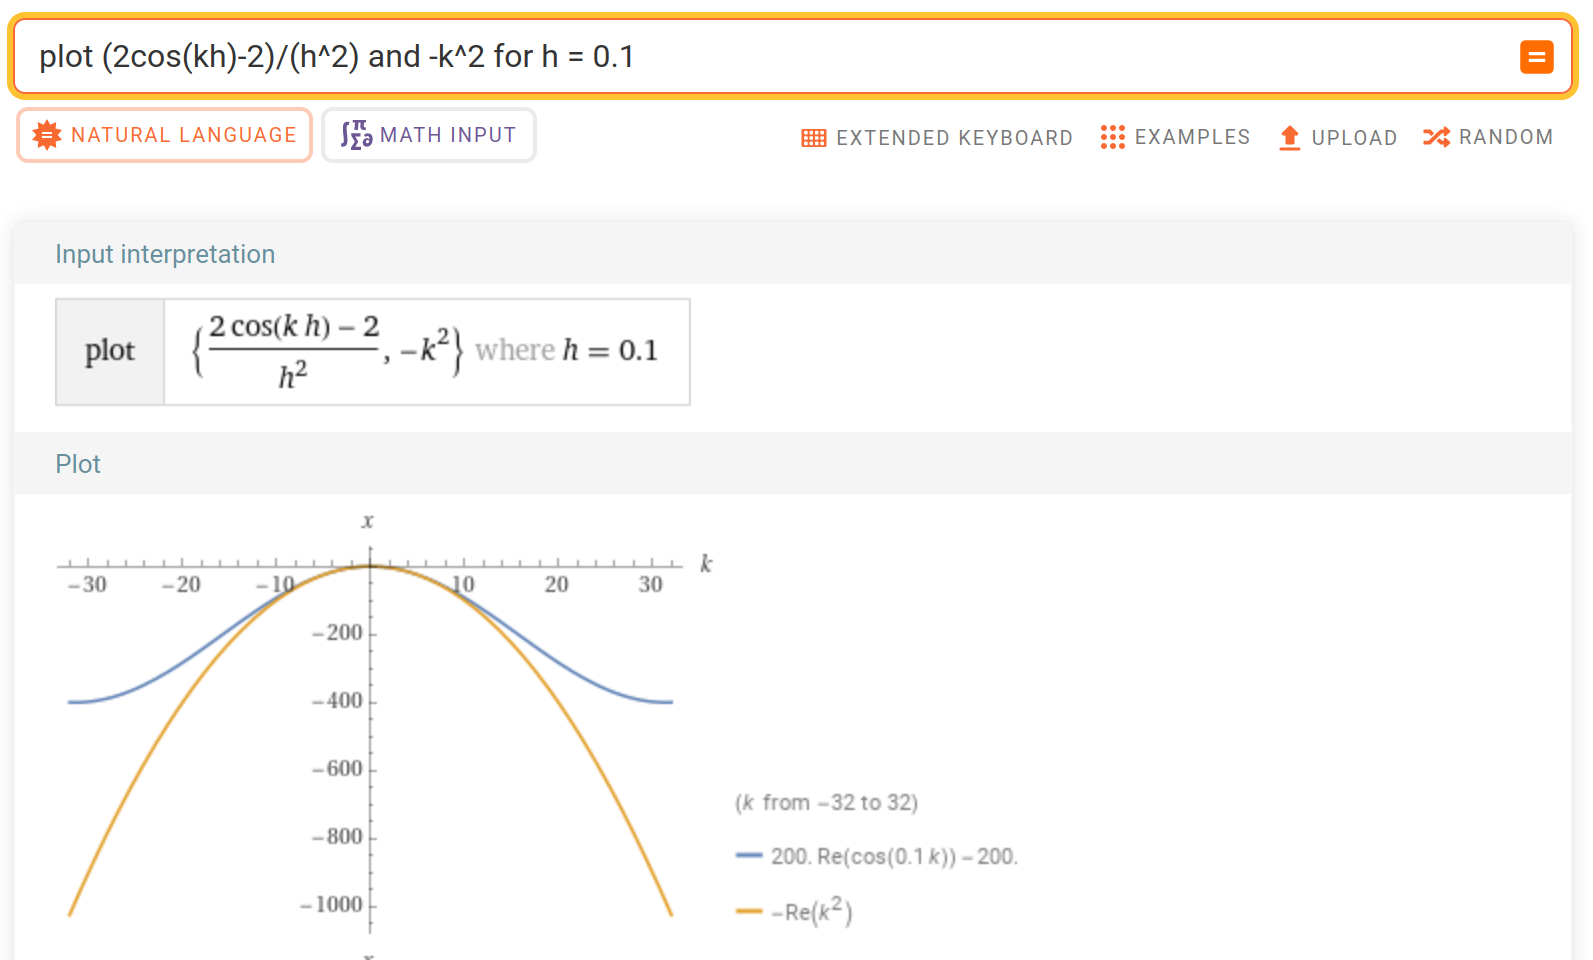
\includegraphics[width=\textwidth]{img/plot1.png}
As one can see both of these look very similar for small k, but diverge as we increase k.

As one can see the plot is symmetric and the expressions do not change if we replace $k$ with $-k$, so we would get the same result for $e^{-\im kx}$, and this for $\cos kx = \frac{1}{2}\left(e^{\im kx} + e^{-\im kx}\right)$.
\end{solution}

\end{document}